%!TEX root = lot1.tex
%--------------------------CARTES PERSONNAGE--------------------------------------------------------------------------------------------

\begin{tikzpicture} %Recto
	%Fond
    \node[anchor=south west,inner sep=0] (carte) at (0,0) {
\includegraphics[width=7.1 cm, height=9.6 cm]{fonds/noir.png}};
    \node[anchor=center] at (carte.center) {
\includegraphics[width=\cardwidth cm, height=\cardheight cm]{fonds/fond_plan.png}};

    %Titre
	\node[anchor=center] at (\titleX,\titleY) {\titlefont Planning};

	%Description
	\node[anchor=north west, text width=5.6cm] (description) at (\descriptionX,8) {\descriptionfont\setsize{11} \begin{enumerate}
\item DSI
\item Stagiaire
\item Manager
\item Marketing
\item PMO
\item Développeur
\item Cryptologue
\item Ingénieur Système
\item {\textit{ Assistante de Direction}}
\end{enumerate}
};

\end{tikzpicture}

\begin{tikzpicture} %Verso
	%Fond
    \node[anchor=south west,inner sep=0] (carte) at (0,0) {
\includegraphics[width=7.1 cm, height=9.6 cm]{fonds/noir.png}};
    \node[anchor=center] at (carte.center) {
\includegraphics[width=\cardwidth cm, height=\cardheight cm]{fonds/fond_plan.png}};

    %Titre
	\node[anchor=center] at (\titleX,\titleY) {\titlefont Planning};

	%Description
	\node[anchor=north west, text width=5.6cm] (description) at (\descriptionX,8) {\descriptionfont\setsize{11} \begin{enumerate}
\item DSI
\item Stagiaire
\item Manager
\item Marketing
\item PMO
\item Développeur
\item Cryptologue
\item Ingénieur Système
\item {\textit {Assistante de Direction}}
\end{enumerate}
};

\end{tikzpicture}



%%%%%%%%%%%%%%%%%%%%%%%%%%%%%%%%%%%%%%%%%%%%%%%%%%%%%%%%%%%%%%

\begin{tikzpicture} %Recto
	%Fond
    \node[anchor=south west,inner sep=0] (carte) at (0,0) {
\includegraphics[width=7.1 cm, height=9.6 cm]{fonds/noir.png}};
    \node[anchor=center] at (carte.center) {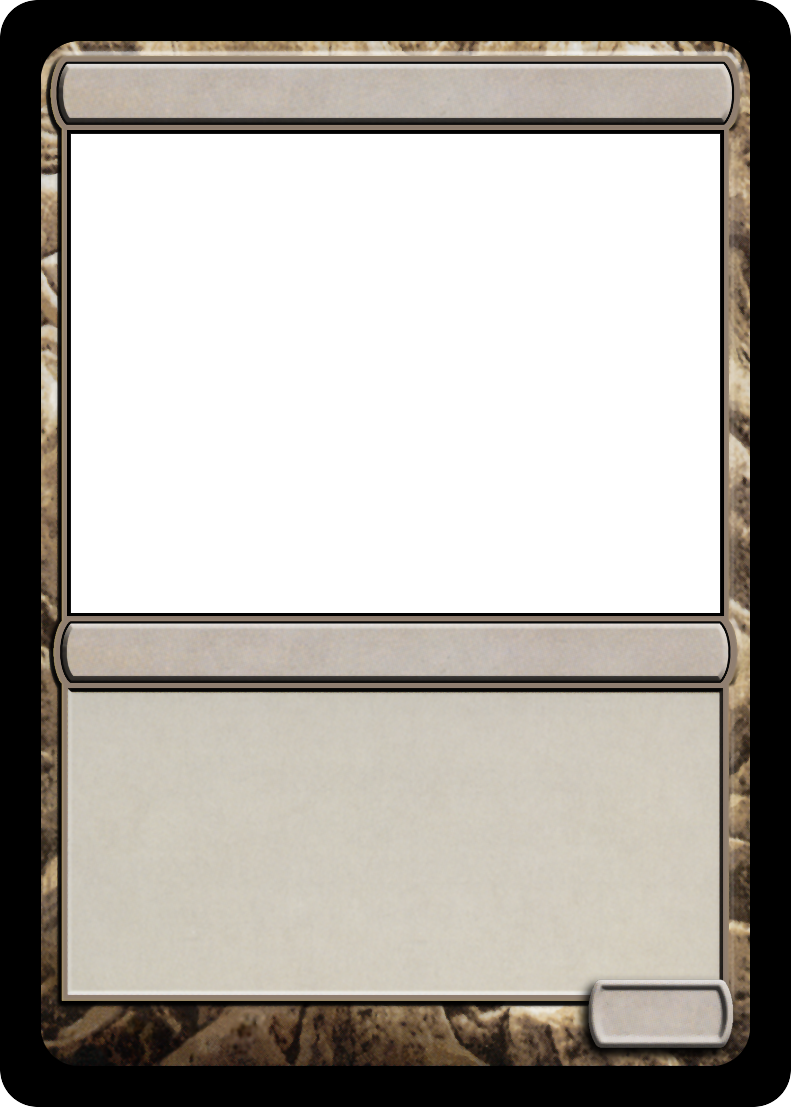
\includegraphics[width=\cardwidth cm, height=\cardheight cm]{fonds/fond_personnage.png}};

    %Titre
	\node[anchor=center] at (\titleX,\titleY) {\titlefont DSI};

	%Image
	\node[anchor=center] at (\imageX,\imageY) {
\includegraphics[width=\imageWidth px, height=\imageHeight px]{images/P1_DSI.png}};
	\node[anchor=center] at (6.1,4.5) {
\includegraphics[width=12 px, height=6 px]{fonds2/legacy.jpg}};

	%Type
	\node[anchor=center] at (\typeX,\typeY) {\typefont Personnage};

	%Description
	\node[anchor=north west, text width=5.6cm] (description) at (\descriptionX,\descriptionY) {\descriptionfont\setsize{6}(Bonus) DSI paralyse un personnage pour ce tour. Le joueur terminera son UO directement sans piocher. Celui-ci doit également écrire le mot ``demande KiSS'' sur un papier pendant que les autres jouent leur UO. Le joueur DSI jettera avec le plus grand mépris la demande à la poubelle.\par};

	%Punchline
	\node[anchor=north west, text width=5.6cm, below = 1pt of description] (punchline) {\punchlinefont\setsize{6}(Permanent) Avant de vous parler, les autres joueurs doivent dire 3915.\par};

	%Separateur !!!!!PAS TOUCHE!!!!!
	\fill[black,path fading=west] (description.south west) rectangle (punchline.north);
	\fill[black,path fading=east] (punchline.north) rectangle (description.south east);

	%Numéro !!!!!PAS TOUCHE!!!!!
	\node[anchor=center] at (\numberX,\numberY) {\numberfont 1/8};
\end{tikzpicture}\versoperso %Verso

%%%%%%%%%%%%%%%%%%%%%%STAGIAIRE%%%%%%%%%%%%%%%%%%%%%%%%%%%%%%%%%%%%%%%%
\begin{tikzpicture} %Recto
	%Fond
    \node[anchor=south west,inner sep=0] (carte) at (0,0) {
\includegraphics[width=7.1 cm, height=9.6 cm]{fonds/noir.png}};
    \node[anchor=center] at (carte.center) {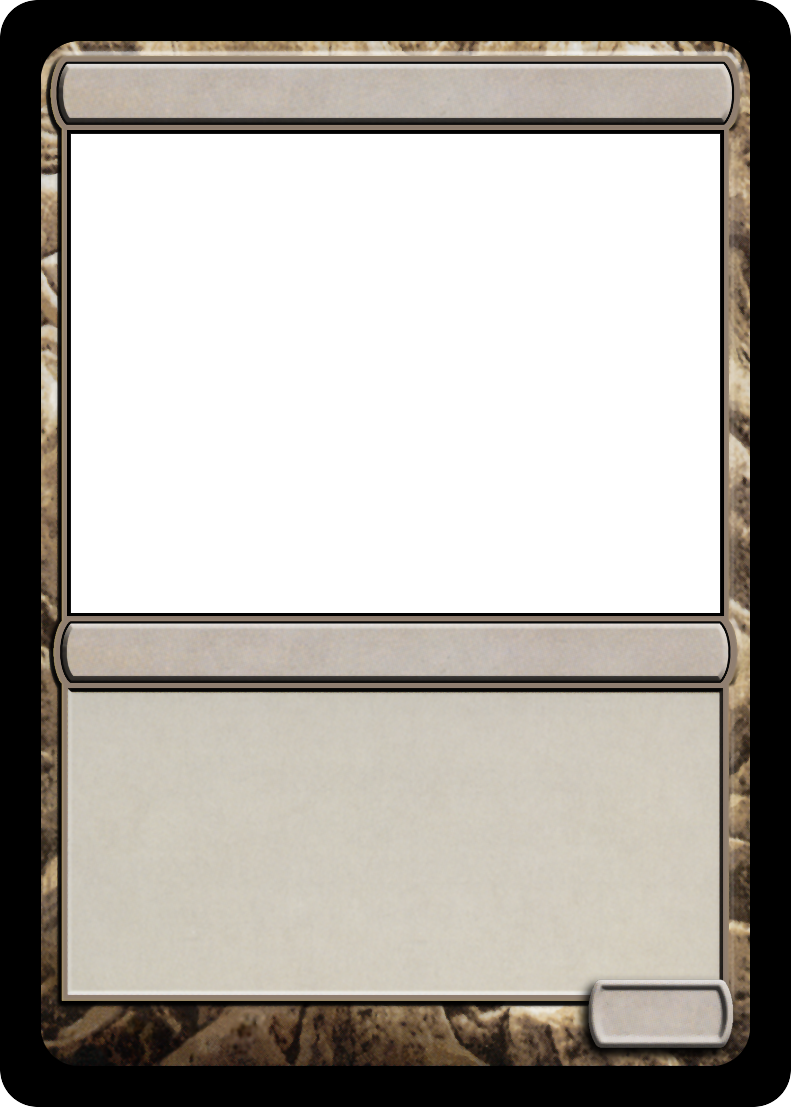
\includegraphics[width=\cardwidth cm, height=\cardheight cm]{fonds/fond_personnage.png}};

    %Titre
	\node[anchor=center] at (\titleX,\titleY) {\titlefont Stagiaire};

	%Image
	\node[anchor=center] at (\imageX,\imageY) {
\includegraphics[width=\imageWidth px, height=\imageHeight px]{images/P2_Stagiaire.jpg}};
	\node[anchor=center] at (6.1,4.5) {
\includegraphics[width=12 px, height=6 px]{fonds2/legacy.jpg}};

	%Type
	\node[anchor=center] at (\typeX,\typeY) {\typefont Personnage};

	%Description
	\node[anchor=north west, text width=5.6cm] (description) at (\descriptionX,\descriptionY) {\descriptionfont\setsize{6}(Bonus) Le stagiaire choisit un joueur autour de la table qui sera son tuteur. Il tire un CDI à pile ou face. En cas de victoire il obtient un tour supplémentaire `nouveau contrat' à la fin du tour avec effet bonus équivalent à celui du tuteur.\par};

	%Punchline
	\node[anchor=north west, text width=5.6cm, below = 1pt of description] (punchline) {\punchlinefont\setsize{5}(Invisibilité) Seul le tuteur peut jouer des cartes malus contre lui. Son tuteur peut lui demander d’aller chercher un café pendant le tour. Les autres joueurs vous appellent ``machin''.\par};

	%Separateur !!!!!PAS TOUCHE!!!!!
	\fill[black,path fading=west] (description.south west) rectangle (punchline.north);
	\fill[black,path fading=east] (punchline.north) rectangle (description.south east);

	%Numéro !!!!!PAS TOUCHE!!!!!
	\node[anchor=center] at (\numberX,\numberY) {\numberfont 2/8};
\end{tikzpicture}\versoperso %Verso

%%%%%%%%%%%%%%%%%%%%%%%%%%%%%%%%%%%%%%%%%%%%%%%%%%%%%%%%%%%%%%

\begin{tikzpicture} %Recto
	%Fond
    \node[anchor=south west,inner sep=0] (carte) at (0,0) {
\includegraphics[width=7.1 cm, height=9.6 cm]{fonds/noir.png}};
    \node[anchor=center] at (carte.center) {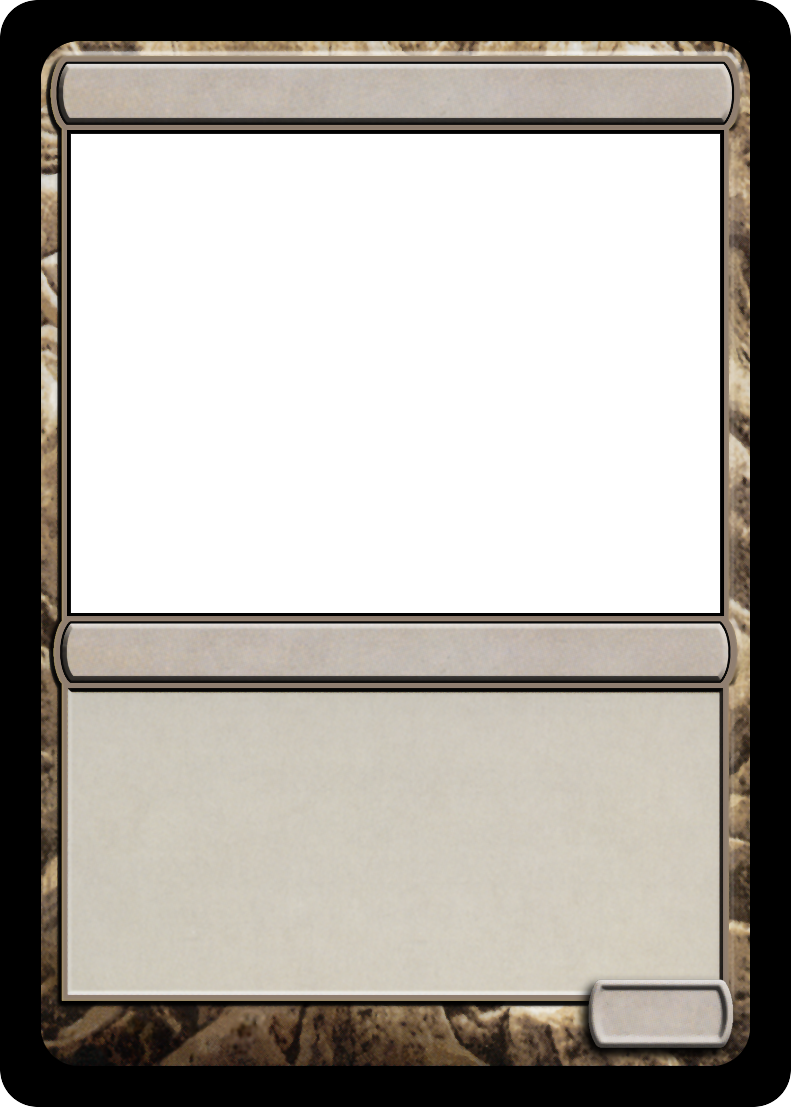
\includegraphics[width=\cardwidth cm, height=\cardheight cm]{fonds/fond_personnage.png}};

    %Titre
	\node[anchor=center] at (\titleX,\titleY) {\titlefont Manager};

	%Image
	\node[anchor=center] at (\imageX,\imageY) {
\includegraphics[width=\imageWidth px, height=\imageHeight px]{images/P3_Manager.jpg}};
	\node[anchor=center] at (6.1,4.5) {
\includegraphics[width=12 px, height=6 px]{fonds2/legacy.jpg}};

	%Type
	\node[anchor=center] at (\typeX,\typeY) {\typefont Personnage};

	%Description
	\node[anchor=north west, text width=5.6cm] (description) at (\descriptionX,\descriptionY) {\descriptionfont\setsize{6}(Délégation) Il peut déléguer une carte de sa main vers un autre personnage de son choix et demander à un joueur d’échanger sa chaise avec un autre. \par};

	%Punchline
	\node[anchor=north west, text width=5.6cm, below = 1pt of description] (punchline) {\punchlinefont\setsize{6}(Directisation) Lorsqu’un joueur peut défausser une carte, révéler une carte, si elle vaut 8 vous directisez (défaussez) à la place du joueur. Les autres joueurs doivent appeler le personnage ``chef''. \par};

	%Separateur !!!!!PAS TOUCHE!!!!!
	\fill[black,path fading=west] (description.south west) rectangle (punchline.north);
	\fill[black,path fading=east] (punchline.north) rectangle (description.south east);

	%Numéro !!!!!PAS TOUCHE!!!!!
	\node[anchor=center] at (\numberX,\numberY) {\numberfont 3/8};
\end{tikzpicture}\versoperso %Verso

%%%%%%%%%%%%%%%%%%%%%%%%%%%%%%%%%%%%%%%%%%%%%%%%%%%%%%%%%%%%%% MARKET
\begin{tikzpicture} %Recto
	%Fond
    \node[anchor=south west,inner sep=0] (carte) at (0,0) {
\includegraphics[width=7.1 cm, height=9.6 cm]{fonds/noir.png}};
    \node[anchor=center] at (carte.center) {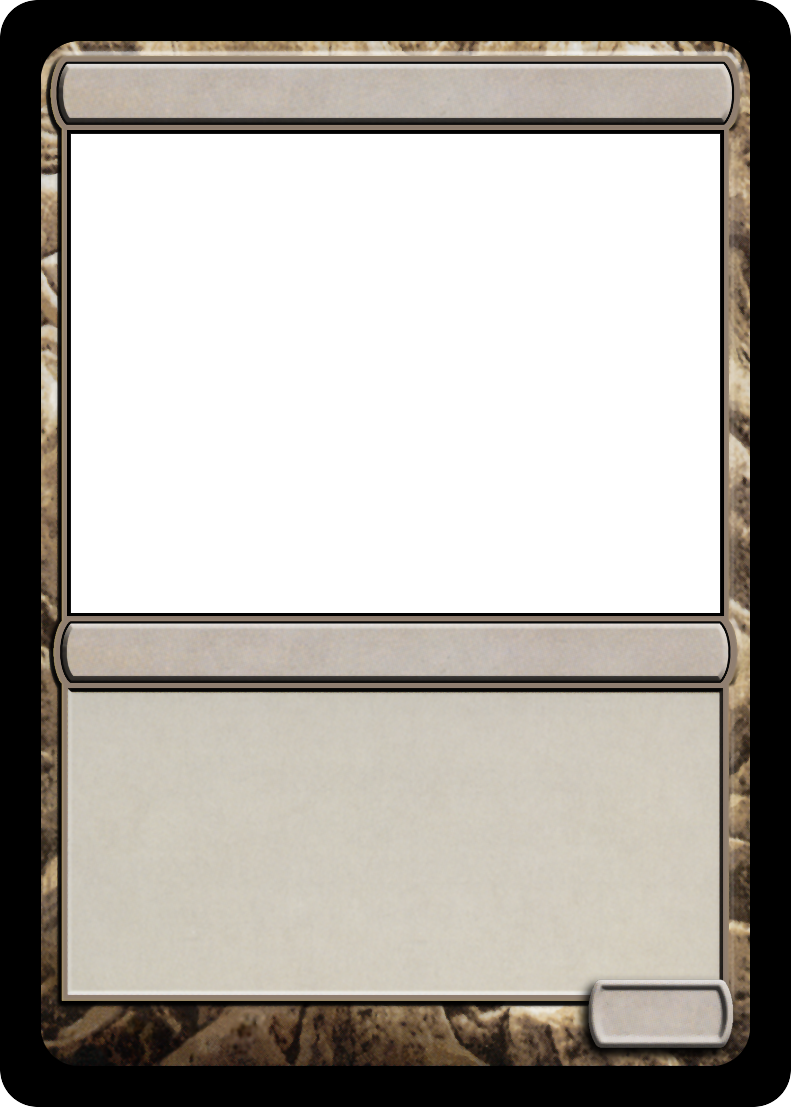
\includegraphics[width=\cardwidth cm, height=\cardheight cm]{fonds/fond_personnage.png}};

    %Titre
	\node[anchor=center] at (\titleX,\titleY) {\titlefont Marketing};

	%Image
	\node[anchor=center] at (\imageX,\imageY) {
\includegraphics[width=\imageWidth px, height=\imageHeight px]{images/P4_Marketting.jpg}};
	\node[anchor=center] at (6.1,4.5) {
\includegraphics[width=12 px, height=6 px]{fonds2/legacy.jpg}};

	%Type
	\node[anchor=center] at (\typeX,\typeY) {\typefont Personnage};

	%Description
	\node[anchor=north west, text width=5.6cm] (description) at (\descriptionX,\descriptionY) {\descriptionfont\setsize{6}(Enfumage) Le marketing peut en*u*er$^1$ le personnage de son choix et échanger jusqu’à 4 cartes de sa main avec des cartes choisies aléatoirement dans celle d’un autre joueur.\par};

	%Punchline
	\node[anchor=north west, text width=5.6cm, below = 1pt of description] (punchline) {\punchlinefont\setsize{6}(Permanent) Les autres joueurs vous méprisent techniquement, mais sont jaloux de vous.\par};

	%Specifique à cette carte
	\node[anchor=north west, text width=5.6cm, below = 1pt of punchline] (footnote) {\descriptionfont\setsize{5}1 : enfumer évidemment. Pervers !\par};

	%Separateur !!!!!PAS TOUCHE!!!!!
	\fill[black,path fading=west] (description.south west) rectangle (punchline.north);
	\fill[black,path fading=east] (punchline.north) rectangle (description.south east);

	%Numéro !!!!!PAS TOUCHE!!!!!
	\node[anchor=center] at (\numberX,\numberY) {\numberfont 4/8};
\end{tikzpicture}\versoperso %Verso

%%%%%%%%%%%%%%%%%%%%%%%%%%%%%%%%%%%%%%%%%%%%%%%%%%%%%%%%%%%%%% PMO
\begin{tikzpicture} %Recto
	%Fond
    \node[anchor=south west,inner sep=0] (carte) at (0,0) {
\includegraphics[width=7.1 cm, height=9.6 cm]{fonds/noir.png}};
    \node[anchor=center] at (carte.center) {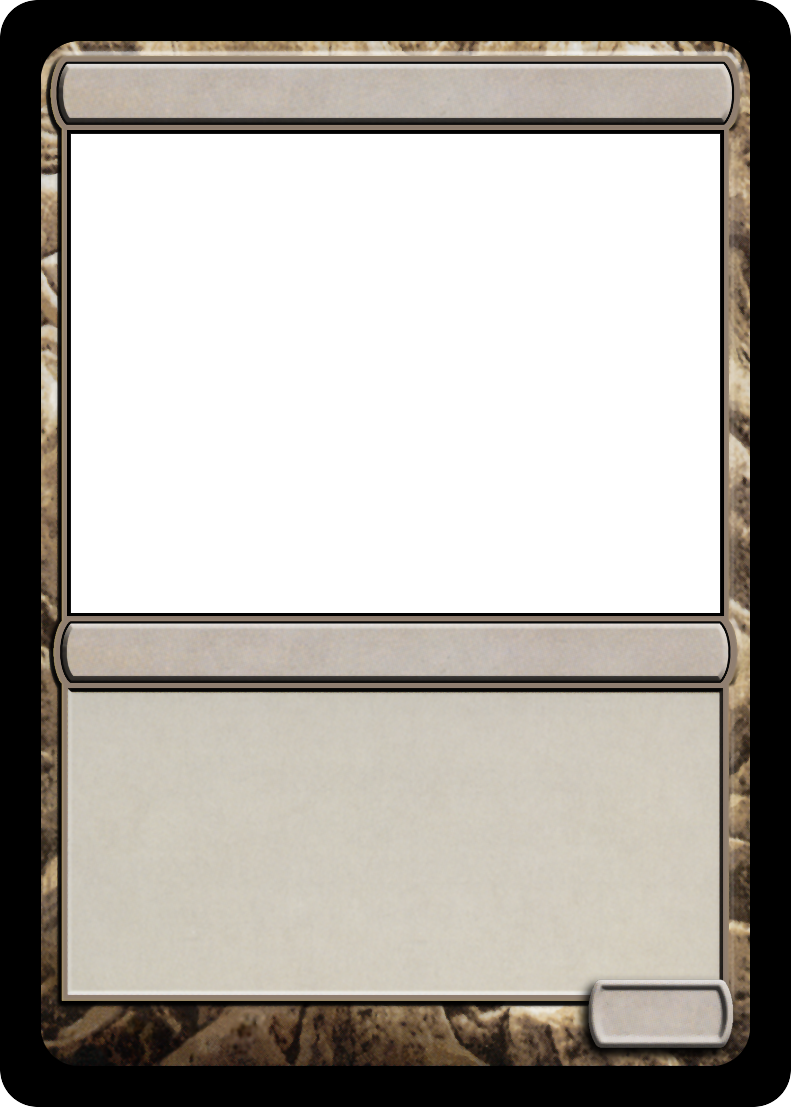
\includegraphics[width=\cardwidth cm, height=\cardheight cm]{fonds/fond_personnage.png}};

    %Titre
	\node[anchor=center] at (\titleX,\titleY) {\titlefont PMO (Gestionnaire)};

	%Image
	\node[anchor=center] at (\imageX,\imageY) {
\includegraphics[width=\imageWidth px, height=\imageHeight px]{images/P5_pmo.jpg}};
	\node[anchor=center] at (6.1,4.5) {
\includegraphics[width=12 px, height=6 px]{fonds2/legacy.jpg}};

	%Type
	\node[anchor=center] at (\typeX,\typeY) {\typefont Personnage ennuyeux};

	%Description
	\node[anchor=north west, text width=5.6cm] (description) at (\descriptionX,\descriptionY) {\descriptionfont\setsize{8}(Planification) Le PMO acquiert la carte planning. Il peut jouer une carte neutre supplémentaire.\par};

	%Punchline
	\node[anchor=north west, text width=5.6cm, below = 1pt of description] (punchline) {\punchlinefont\setsize{8}(Permanent) Les autres joueurs ne vous écoutent pas attentivement durant ce tour.\par};

	%Separateur !!!!!PAS TOUCHE!!!!!
	\fill[black,path fading=west] (description.south west) rectangle (punchline.north);
	\fill[black,path fading=east] (punchline.north) rectangle (description.south east);

	%Numéro !!!!!PAS TOUCHE!!!!!
	\node[anchor=center] at (\numberX,\numberY) {\numberfont 5/8};
\end{tikzpicture}\versoperso %Verso

%%%%%%%%%%%%%%%%%%%%%%%%%%%% PERSONNAGE ELECTRONICIEN
\begin{tikzpicture} %Recto
	%Fond
    \node[anchor=south west,inner sep=0] (carte) at (0,0) {
\includegraphics[width=7.1 cm, height=9.6 cm]{fonds/noir.png}};
    \node[anchor=center] at (carte.center) {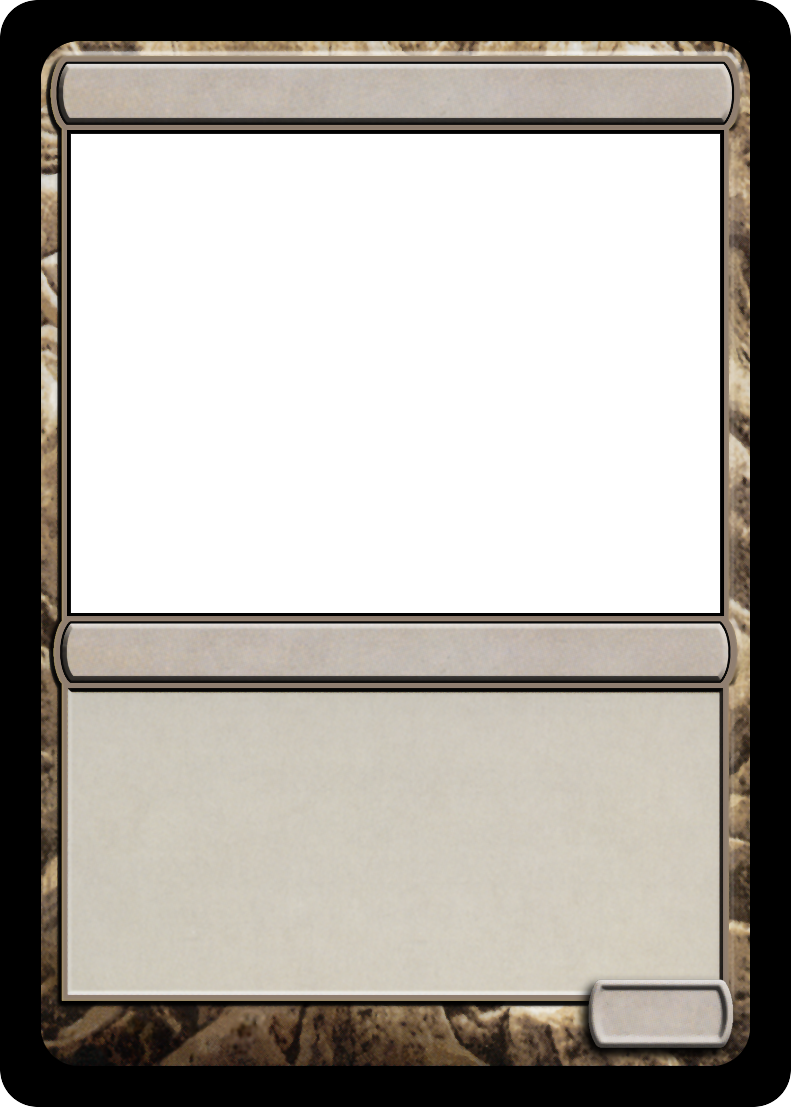
\includegraphics[width=\cardwidth cm, height=\cardheight cm]{fonds/fond_personnage.png}};

    %Titre
	\node[anchor=center] at (\titleX,\titleY) {\titlefont Composant (\'Electronicien) };

	%Image
	\node[anchor=center] at (\imageX,\imageY) {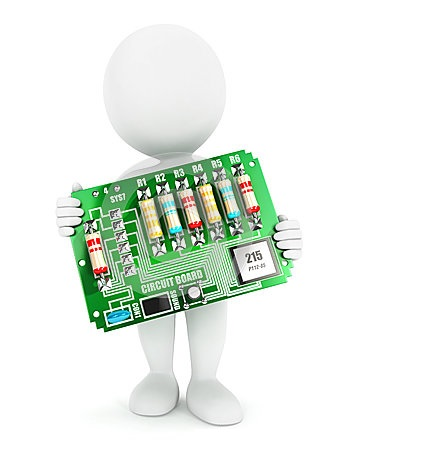
\includegraphics[width=\imageWidth px, height=\imageHeight px]{images/P9_compo.png}};
	\node[anchor=center] at (6.1,4.5) {
\includegraphics[width=12 px, height=6 px]{fonds2/legacy.jpg}};

	%Type
	\node[anchor=center] at (\typeX,\typeY) {\typefont Personnage };

	%Description
	\node[anchor=north west, text width=5.6cm] (description) at (\descriptionX,\descriptionY) {\descriptionfont\setsize{6}(VHDL) Le joueur dessine des petits créneaux sur une feuille puis révèle une carte du tas. En cas de parité identique avec le nombre de créneaux, le routage fonctionne et le personnage peut imputer deux cartes supplémentaires. \par};

	%Punchline
	\node[anchor=north west, text width=5.6cm, below = 1pt of description] (punchline) {\punchlinefont\setsize{6}(Outre-espace) Vous vivez aux confins lointains de la zone et devez vous asseoir à l'opposé de la table par rapport au cryptologue à ce tour.\par};

	%Separateur !!!!!PAS TOUCHE!!!!!
	\fill[black,path fading=west] (description.south west) rectangle (punchline.north);
	\fill[black,path fading=east] (punchline.north) rectangle (description.south east);

	%Numéro !!!!!PAS TOUCHE!!!!!
	\node[anchor=center] at (\numberX,\numberY) {\numberfont 6/8};
\end{tikzpicture}\versoperso %Verso

%%%%%%%%%%%%%%%%%%%%%%%%%%%%%%%%%%%%%%%%%%%%%%%%%%%%%%%%%%%%%% 7: CRYPTOLOGUE
\begin{tikzpicture} %Recto
	%Fond
    \node[anchor=south west,inner sep=0] (carte) at (0,0) {
\includegraphics[width=7.1 cm, height=9.6 cm]{fonds/noir.png}};
    \node[anchor=center] at (carte.center) {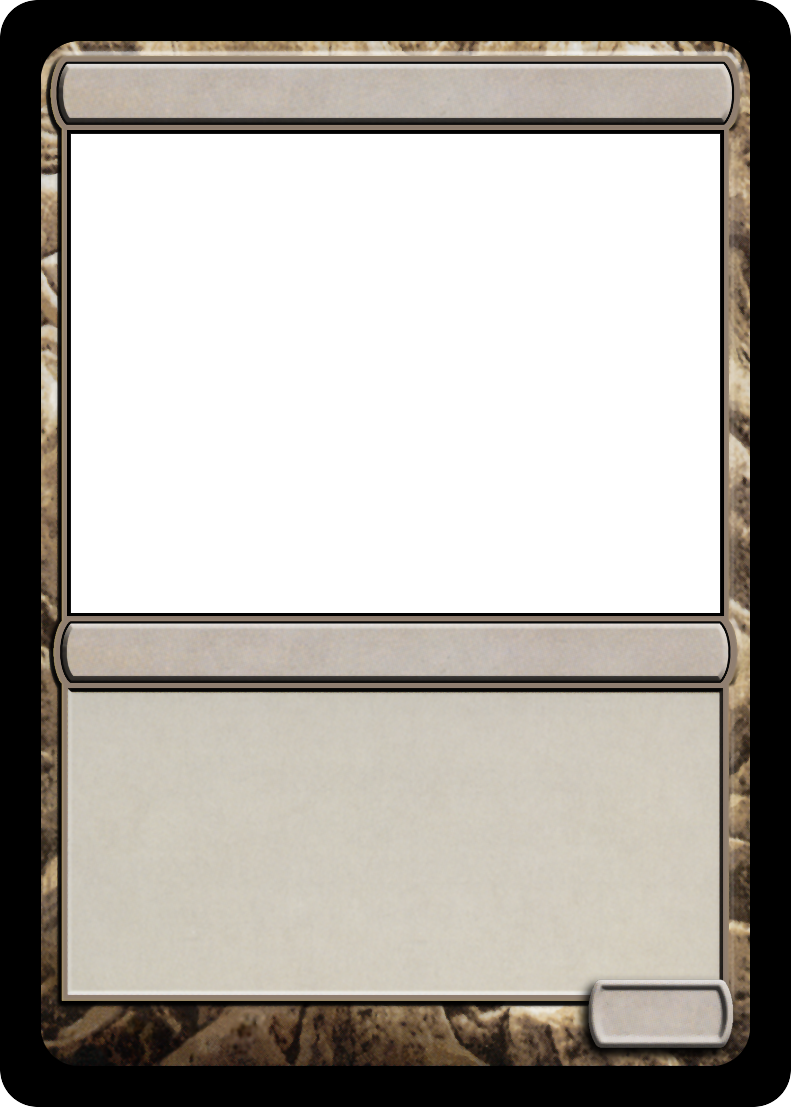
\includegraphics[width=\cardwidth cm, height=\cardheight cm]{fonds/fond_personnage.png}};

    %Titre
	\node[anchor=center] at (\titleX,\titleY) {\titlefont Cryptologue};

	%Image
	\node[anchor=center] at (\imageX,\imageY) {
\includegraphics[width=\imageWidth px, height=\imageHeight px]{images/P7_Cryptologue.jpg}};
	\node[anchor=center] at (6.1,4.5) {
\includegraphics[width=12 px, height=6 px]{fonds2/legacy.jpg}};

	%Type
	\node[anchor=center] at (\typeX,\typeY) {\typefont Personnage};

	%Description
	\node[anchor=north west, text width=5.6cm] (description) at (\descriptionX,\descriptionY) {\descriptionfont\setsize{8}(Astucieux) Le cryptologue pioche deux cartes puis défausse deux cartes. Il peut également imputer une carte supplémentaire.\par};

	%Punchline
	\node[anchor=north west, text width=5.6cm, below = 1pt of description] (punchline) {\punchlinefont\setsize{8}(Génial) Les autres joueurs vous admirent secrètement durant ce tour. \par};

	%Separateur !!!!!PAS TOUCHE!!!!!
	\fill[black,path fading=west] (description.south west) rectangle (punchline.north);
	\fill[black,path fading=east] (punchline.north) rectangle (description.south east);

	%Numéro !!!!!PAS TOUCHE!!!!!
	\node[anchor=center] at (\numberX,\numberY) {\numberfont 7/8};
\end{tikzpicture}\versoperso %Verso

%%%%%%%%%%%%%%%%%%%%%%%%%%%%%%%%%%%%%%%%%%%%%%%%%%%%%%%%%%%%%% 8: IS
\begin{tikzpicture} %Recto
	%Fond
    \node[anchor=south west,inner sep=0] (carte) at (0,0) {
\includegraphics[width=7.1 cm, height=9.6 cm]{fonds/noir.png}};
    \node[anchor=center] at (carte.center) {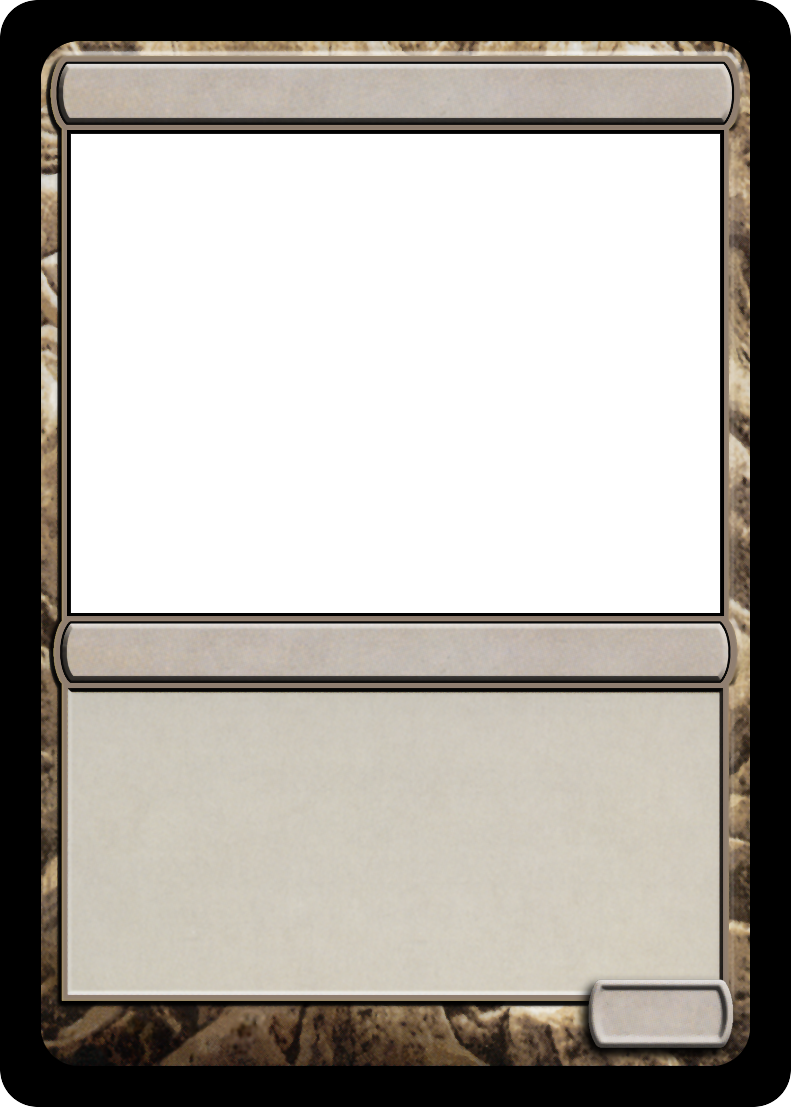
\includegraphics[width=\cardwidth cm, height=\cardheight cm]{fonds/fond_personnage.png}};

    %Titre
	\node[anchor=center] at (\titleX,\titleY) {\titlefont Ingénieur Système};

	%Image
	\node[anchor=center] at (\imageX,\imageY) {
\includegraphics[width=\imageWidth px, height=\imageHeight px]{images/P8_IS.png}};
	\node[anchor=center] at (6.1,4.5) {
\includegraphics[width=12 px, height=6 px]{fonds2/legacy.jpg}};

	%Type
	\node[anchor=center] at (\typeX,\typeY) {\typefont Personnage};

	%Description
	\node[anchor=north west, text width=5.6cm] (description) at (\descriptionX,\descriptionY) {\descriptionfont\setsize{8}(Bonus) Au début de son tour l’ingénieur système force un autre joueur de son choix à piocher une carte. L’ingénieur système remet toujours tout en cause et peut jouer une carte malus (ou côté spécifique malus) supplémentaire.\par};

	%Punchline
	\node[anchor=north west, text width=5.6cm, below = 1pt of description] (punchline) {\punchlinefont\setsize{7}(Permanent) Tout le monde vous déteste, même Gandhi (si, si !).\par};

	%Separateur !!!!!PAS TOUCHE!!!!!
	\fill[black,path fading=west] (description.south west) rectangle (punchline.north);
	\fill[black,path fading=east] (punchline.north) rectangle (description.south east);

	%Numéro !!!!!PAS TOUCHE!!!!!
	\node[anchor=center] at (\numberX,\numberY) {\numberfont 8/8};
\end{tikzpicture}\versoperso %Verso

%%%%%%%%%%%%%%%%%%%%%%%%%%%%%%%%%%%%%%%%%%%%%%%%%%%%%%%%%%%%%% 9: Assistante
\begin{tikzpicture} %Recto
	%Fond
    \node[anchor=south west,inner sep=0] (carte) at (0,0) {
\includegraphics[width=7.1 cm, height=9.6 cm]{fonds/noir.png}};
    \node[anchor=center] at (carte.center) {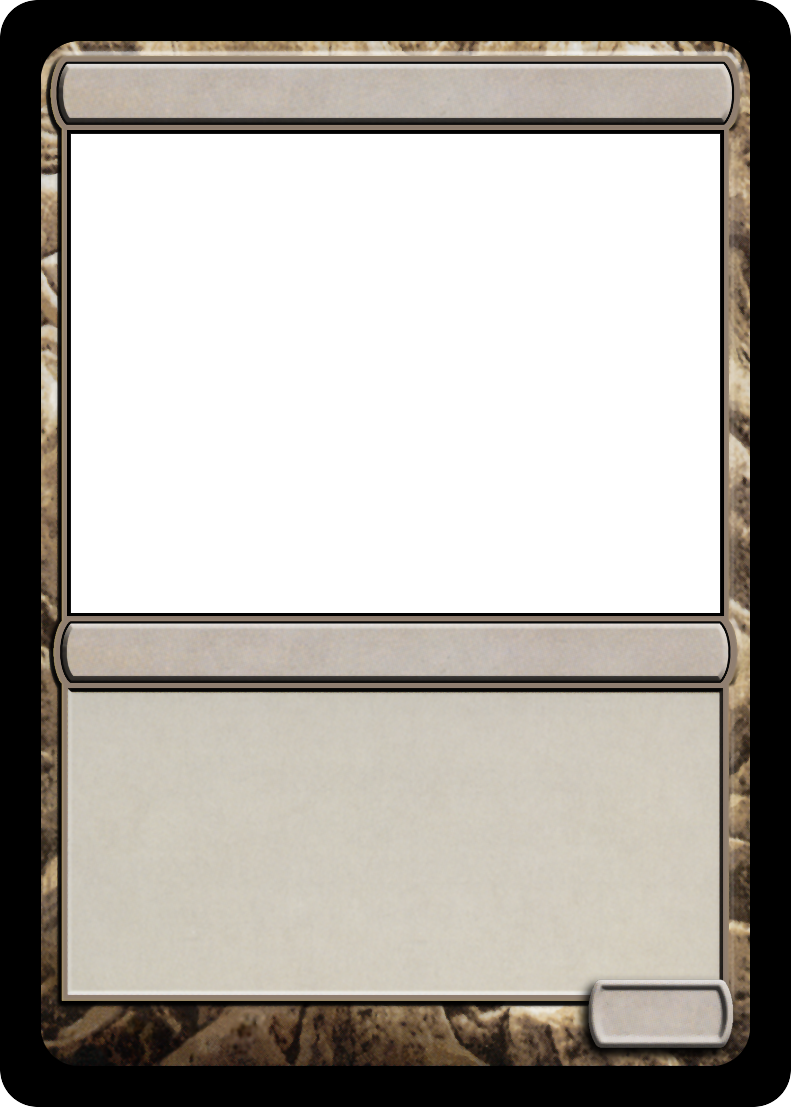
\includegraphics[width=\cardwidth cm, height=\cardheight cm]{fonds/fond_personnage.png}};

    %Titre
	\node[anchor=center] at (\titleX,\titleY) {\titlefont Assistante de Direction};

	%Image
	\node[anchor=center] at (\imageX,\imageY) {
\includegraphics[width=\imageWidth px, height=\imageHeight px]{images/P9_assistante.jpg}};
	\node[anchor=center] at (6.1,4.5) {
\includegraphics[width=12 px, height=6 px]{fonds2/legacy.jpg}};

	%Type
	\node[anchor=center] at (\typeX,\typeY) {\typefont Personnage};

	%Description
	\node[anchor=north west, text width=5.6cm] (description) at (\descriptionX,\descriptionY) {\descriptionfont\setsize{8}(Bonus) Au début de son tour, si l'assistante est assise a côté du manager, elle se défausse immédiatement de deux cartes.\par};

	%Punchline
	\node[anchor=north west, text width=5.6cm, below = 1pt of description] (punchline) {\punchlinefont\setsize{7}(Permanent) ``Il est très occupé. Le déjeuner du COPIL précède le cocktail du CODIR"\par};

	%Separateur !!!!!PAS TOUCHE!!!!!
	\fill[black,path fading=west] (description.south west) rectangle (punchline.north);
	\fill[black,path fading=east] (punchline.north) rectangle (description.south east);

	%Numéro !!!!!PAS TOUCHE!!!!!
	\node[anchor=center] at (\numberX,\numberY) {\numberfont 9/9};
\end{tikzpicture}\versoperso %Verso

%--------------------------CARTES SPECIALES------------------------------------------------------------------------------------------------ ANSSI
\begin{tikzpicture} %Recto
	%Fond
    \node[anchor=south west,inner sep=0] (carte) at (0,0) {
\includegraphics[width=7.1 cm, height=9.6 cm]{fonds/noir.png}};
    \node[anchor=center] at (carte.center) {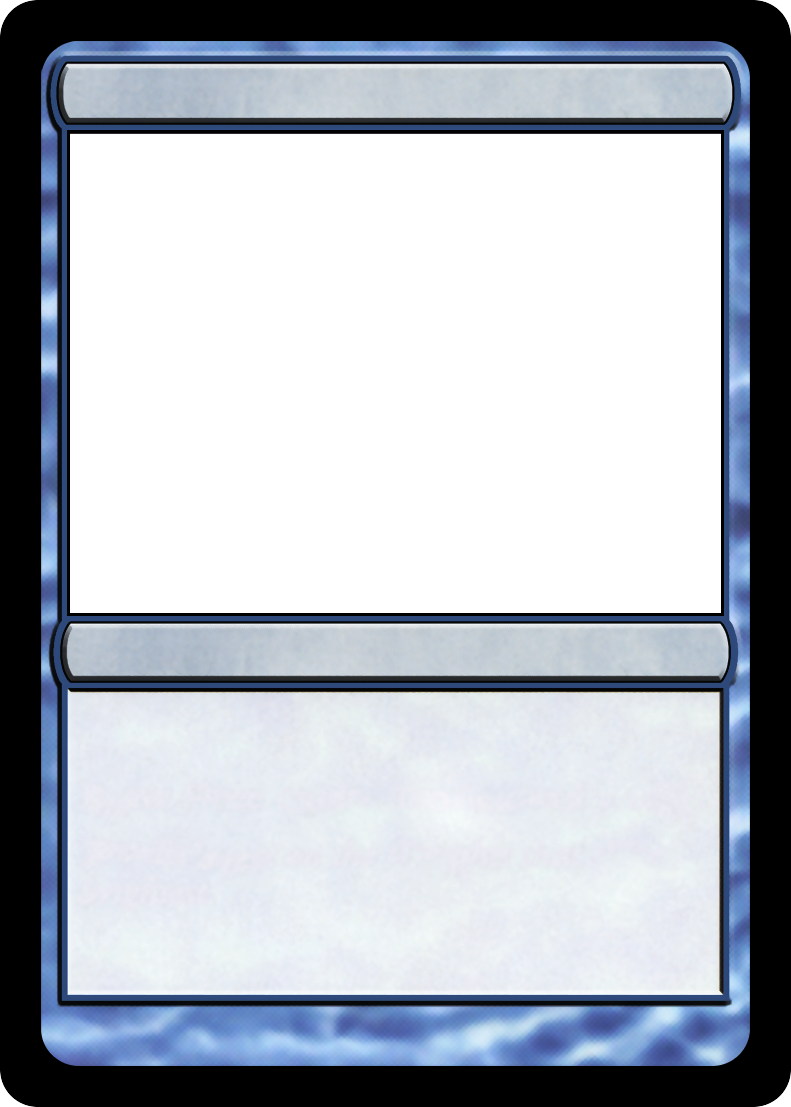
\includegraphics[width=\cardwidth cm, height=\cardheight cm]{fonds/fond_anssi.png}};

    %Titre
	\node[anchor=center] at (\titleX,\titleY) {\titlefont ANSSI};

	%Image
	\node[anchor=center] at (\imageX,\imageY) {
\includegraphics[width=\imageWidth px, height=\imageHeight px]{images/48_ANSSI.png}};
	\node[anchor=center] at (6.1,4.5) {
\includegraphics[width=12 px, height=6 px]{fonds2/legacy.jpg}};

	%Type
	\node[anchor=center] at (\typeX,\typeY) {\typefont Spécial (Permanent)};

	%Description
	\node[anchor=north west, text width=5.6cm] (description) at (\descriptionX,\descriptionY) {\descriptionfont\setsize{6} Placez cette carte devant vous seulement si vous êtes cryptologue. A chaque tour que vous débutez, révélez une carte, si vous ne commetez pas d'impair (la carte est paire) faites pivoter l'ANSSI d'un quart de tour (sens horaire). Après une rotation complète vous gagnez la partie.\par};

	%Punchline
	\node[anchor=north west, text width=5.6cm, below = 1pt of description] (punchline) {\punchlinefont\setsize{6} Convoitée par tous les joueurs, ne rêvez pas, à  moins de tricher, vous ne l'atteindrez  jamais.\par};

	%Separateur !!!!!PAS TOUCHE!!!!!
	\fill[black,path fading=west] (description.south west) rectangle (punchline.north);
	\fill[black,path fading=east] (punchline.north) rectangle (description.south east);
\end{tikzpicture}\verso %Verso
